\documentclass[assignment02_Solutions]{subfiles}

\invalidatemargin

\IfSubStr{\jobname}{\detokenize{Solutions}}{\toggletrue{solutions}}{\togglefalse{solutions}}

\fancypagestyle{firstpage}

{\rhead{Assignment 2 \linebreak \textit{Version: \today}}}

\title{Assignment 2: Probabilistic Graphical Models}
\author{Machine Learning}
\date{Fall 2019}

\begin{document}

\maketitle
\thispagestyle{firstpage}


\begin{learningobjectives}
\bi
\item The concept of independence and conditional independence
\item The basic components of a Bayesian Networks (BN)
\item The rules of d-separation to compute conditional independence relationships in a BN
\item The Compas recidivism risk algorithm controversy
\ei
\end{learningobjectives}

\section{Motivation and Context}
In the last assignment we learned the basic definition of a probability and acquired some very powerful rules for working with probabilities.  In this assignment you'll be taking these ideas and extending them in the following significant ways.

\bi
\item You'll learn a graphical way to represent the relationships between probabilities that will make it much easier to work with large probabilistic models.
\item You'll be taking the ideas of probability using them to derive a whole new way of approaching the classification problem in machine learning.
\ei


\section{Product Rule and Marginalization for Random Variables}
\begin{recall}[Product Rule and Marginalization for Events]
Last assignment we learned about two very powerful techniques for computing the probability of events.
\bi
\item We learned the product rule (or conjunction rule), which states that for any two events $\mathcal{A}$ and $\mathcal{B}$,
\begin{align}
p(\mathcal{A}, \mathcal{B}) &= p(\mathcal{A}) p(\mathcal{B}|\mathcal{A}) \label{eq:prodcutruleevents} \\
&= p(\mathcal{B}) p(\mathcal{A}|\mathcal{B}) \enspace  . \nonumber
\end{align}
\item We learned the rule of marginalization, which states that for any two events $\mathcal{A}$ and $\mathcal{B}$,
\begin{align}
p(\mathcal{A}) &= p(\mathcal{A}, \mathcal{B}) + p(\mathcal{A}, \neg \mathcal{B}) \label{eq:marginalizationevents} \enspace .
\end{align}
\ei
It turns out that these rules can modified slightly to apply to random variables as well (instead of just events).
\end{recall}


\subsection{Product Rule for Random Variables}
Suppose we have two random variables $X$ and $Y$.  If we want to know the probability of random variable $X$ taking on value $x$ (it is common to use a lower case letter to refer to a particular value of a random variable) and random variable $Y$ simultaneously taking on value $y$, we can decompose the joint probability (the probability of both of these things occurring simultaneously) using the product rule.

\begin{align}
p(X = x, Y = y) &= p(X=x)p(Y=y | X=x) & \mbox{or equivalently,}\\
&= p(Y=y)p(X=x|Y=y) \nonumber
\end{align}

Notice that this looks pretty much identical to Equation~\ref{eq:prodcutruleevents} except that instead of referencing whether an event happens, we are now referencing a random variable taking on a particular value.

\begin{notice}
It's very common to use the shorthand $p(x, y)$ to refer to $p(X = x, Y = y)$.  The motivation for this shorthand is that it is obvious from the context that $p(x, y)$ really means the probability of random variable $X$ taking on value $x$ and random variable $Y$ taking on value $y$.  In this assignment we're going to avoid using this shorthand, but we will start using the shorthand in future assignments (we'll warn you when we start using it).  Also, you may see this notation used in external resources, so it helps to know about it.
\end{notice}

\subsection{Marginalization for Random Variables}
Again, suppose we have two random variables $X$ and $Y$.  We are interested in computing $p(X = x)$, but suppose it is difficult to compute this probability directly.  Just as we did for events in the last assignment, we can compute $p(X=x)$ by marginalizing out the random variable $Y$.  For simplicity, let's assume that $Y$ can only take on integer values from 1 to $k$.  We can write the marginal distribution $p(X=x)$ in the following way.

\begin{align}
p(X=x) &= \sum_{y=1}^k p(X=x, Y=y)\label{eq:rvmarginal}
\end{align}

You should notice that this equation is very similar to Equation~\ref{eq:marginalizationevents} except that instead of summing over the probability for the two possible outcomes with respect to the event $\mathcal{B}$ (i.e., $\mathcal{B}$ either happens or it does not), we are now summing over the $k$ possible values that $Y$ could take.  Random variables don't necessarily have to take on values from 1 to $k$.  In general, if the random variable $Y$ can take on any value from some discrete set of values $\mathcal{Y}$ (we are using the calligraphic font because we are referring to a set), then the marginal distribution of $X$ can be written as:
\begin{align}
p(X=x) &= \sum_{y \in \mathcal{Y}} p(X=x, Y=y) \enspace . \label{eq:rvmarginalgeneral}
\end{align}
Notice that Equation~\ref{eq:rvmarginal} is a special case of Equation~\ref{eq:rvmarginalgeneral} where $\mathcal{Y} = \{1, 2, \ldots, k\}$.

\begin{exercise}[(15 minutes)]
This exercise is from the \href{https://en.wikipedia.org/wiki/Marginal_distribution\#Real-world_example}{Wikipedia article on marginal distribution}.

\vspace{1em}

\begin{notice}
Strictly speaking a random variable only takes on real numbers as its value (i.e., a random variable cannot take on the value of ``blue'').  That said, it's common to see folks bend this rule a bit by allowing the random variable to take on values that are not real numbers (e.g., you will see that in the Wikipedia article linked above).  Allowing for random variables to have non-numeric values doesn't really change the math except it makes it meaningless to compute quantities such as the mean.  Since in many cases allowing random variables to take on non-numeric values will make things clearer, we will allow this in our materials.
\end{notice} 
\vspace{1em}

Suppose you want to compute the probability that a pedestrian will be hit by a car, while crossing the road at a pedestrian crossing, without paying attention to the traffic light (a bit morbid, we know).  Let $H$ be a discrete random variable taking on the value ``$\mbox{hit}$'' if the pedestrian is struck and ``$\mbox{not hit}$'' if the pedestrian makes it safely across.  Let $L$ (for traffic light) be a discrete random variable taking on the value ``$\mbox{red}$'' when the light is red, ``$\mbox{yellow}$'' when the light is yellow, and ``$\mbox{green}$'' when the light is green.

The model that governs the prior probability of the light ($L$) is as follows.
\begin{align}
p(L = \mbox{red}) = 0.2 \nonumber \\
p(L = \mbox{yellow}) = 0.1 \nonumber \\
p(L = \mbox{green}) = 0.7
\end{align}
The model that governs the conditional probability of $H$ given $L$ is as follows.
\begin{align}
p(H = \mbox{hit} | L = \mbox{red}) = 0.01 \nonumber \\
p(H = \mbox{not hit} | L = \mbox{red}) = 0.99 &~~~~\mbox{Note: the probability of ``not hit'' is always 1 - probability of hit} \nonumber \\
p(H = \mbox{hit} | L = \mbox{yellow}) = 0.1 \nonumber \\
p(H = \mbox{not hit} | L = \mbox{yellow}) = 0.9 \nonumber \\
p(H = \mbox{hit} | L = \mbox{green}) = 0.8  \nonumber \\
p(H = \mbox{not hit} | L = \mbox{green}) = 0.2 \nonumber
\end{align}

What is $p(H=\mbox{hit})$?

\begin{boxedsolution}
\begin{align}
p(H = \mbox{hit}) &= p(H = \mbox{hit}, L = \mbox{red}) +  p(H = \mbox{hit}, L = \mbox{yellow}) +  p(H = \mbox{hit}, L = \mbox{green}) &\mbox{marginalization} \nonumber \\
&= p(L = \mbox{red}) p(H = \mbox{hit} | L = \mbox{red}) + p(L = \mbox{yellow}) p(H = \mbox{hit} | L = \mbox{yellow}) &\mbox{product rule}\nonumber \\
&\hspace{0.5in}+ p(L = \mbox{green}) p(H = \mbox{hit} | L = \mbox{green}) \nonumber\\
&= (0.2 \times 0.01) + (0.1 \times 0.1) + (0.7 \times 0.8) \nonumber \\
&= 0.572 \nonumber
\end{align}
\end{boxedsolution}
\end{exercise}

\section{Some Twists on Bayes' Rule}

By now hopefully you are starting to feel comfortable with the vanilla form of Bayes' rule.  There are a few quite useful variants that we'd like to point out.  There are no exercises for you to do here, just add these to your bag of tricks (you'll be leveraging them later in this assignment, so you'll have a chance to solidify them then).

\begin{align}
p(\mathcal{A} | \mathcal{B}) &= \frac{p(\mathcal{B}|\mathcal{A}) p(\mathcal{A})}{p(\mathcal{B})} & \mbox{as a reminder, here is vanilla Bayes' rule} \\
p(\mathcal{A}, \mathcal{B} | \mathcal{C}) &= \frac{p(\mathcal{C}|\mathcal{A}, \mathcal{B}) p(\mathcal{A, B})}{p(\mathcal{C})} & \mbox{you can bring over multiple events} \\
p(\mathcal{A} | \mathcal{B}, \mathcal{C}) &= \frac{p(\mathcal{B} | \mathcal{A}, \mathcal{C}) p(\mathcal{A}|\mathcal{C})}{p(\mathcal{B}|\mathcal{C})} & \mbox{you can leave an event to the right of the conditioning bar}
\end{align}

\section{Independence and Conditional Independence}

Two of the most important concepts in probability theory are independence and the closely related concept of conditional independence.  these ideas are important because they let you analyze probabilistic quantities in isolation.  For instance, if you know that two events that you are interested in predicting are independent of each other, then you can make a model of each event in isolation.  This saves makes your life much, much easier since you don't have to consider how the two events interact.  Next, we'll make this high-level idea precise.

\subsection{Independence}
The product rule of probability can be simplified when two events, $\mathcal{A}$ and $\mathcal{B}$ are independent.  As an example, suppose $\mathcal{A}$ represents the event that the first flip of a coin comes up heads and event $\mathcal{B}$ is the event that the second flip of the same coin comes up heads.  Since whether or not $\mathcal{A}$ occurs tells us nothing about whether $\mathcal{B}$ would occur, we say that $\mathcal{A}$ and $\mathcal{B}$ are independent events (we use the notation $\mathcal{A} \condindep \mathcal{B}$ to indicate that $\mathcal{A}$ is independent of $\mathcal{B}$).  An event $\mathcal{A}$ is independent of another event $\mathcal{B}$ if and only if the following condition holds.
\begin{align}
p(\mathcal{A}, \mathcal{B}) &= p(\mathcal{A}) p(\mathcal{B}) \label{eq:indepevents}
\end{align}

A direct consequence of Equation~\ref{eq:indepevents} is that if $\mathcal{A} \condindep \mathcal{B}$, then
\begin{align}
p(\mathcal{A} | \mathcal{B}) &= p(\mathcal{A}) & \mbox{and} \nonumber \\
p(\mathcal{B} | \mathcal{A}) &= p(\mathcal{B}) \enspace . \nonumber
\end{align}

A very similar equation to Equation~\ref{eq:indepevents} can be defined for random variables.  Two random variables $X$ and $Y$ are independent if and only if the following condition holds for any values $x$ and $y$.

\begin{align}
p(X=x, Y=y) &= P(X=x) p(Y=y)
\end{align}
Similar to the rule for events, $p(X=x | Y=y) = P(X=x)$ if $X \condindep Y$.

\begin{exercise}[(10 minutes)]
\bes
\item Provide at least 3 examples of events or random variables that are independent of each other.

\begin{boxedsolution}
\bi
\item The event that a coin comes up heads on the first throw and the event that the coin comes up heads on the second throw.
\item A random variable that represents that last digit on a car's license plate and a random variable that represents the last digit on another car's license plate.
\item The event that captures whether or not it rains tomorrow in Boston and a random variable that represents the number of people who attend a rock concert in California tomorrow night (at least it seems that these things are unrelated).
\ei
\end{boxedsolution}

\item Provide at least 3 examples of events or random variables that are not independent of each other.

\begin{boxedsolution}
Here are some ideas.
\bi
\item The daily increase in the Dow Jones Industrial average and the daily increase in the NASDAQ.
\item The event that the American League wins the World Series in 2019 and the event that the National League wins the World Series in 2019.
\item Testing positive for a disease and having that disease.
\ei
\end{boxedsolution}

\ees
\end{exercise}

\subsection{Conditional Independence}
Sometimes two events (or two random variables) that are not independent might become independent when conditioned on another event.

\begin{exercise}[(20 minutes)]

As a motivating example for the concept of conditional independence, consider a variant of the coin problem we saw last assignment.  A bag contains two coins.  Suppose we choose one of the two coins with equal probability.  Let $\mathcal{C}_1$ represents the event that we choose coin 1 and $\mathcal{C}_2$ represent the event that we choose coin 2.  Coin 1 is fair $p(\mathcal{H} | \mathcal{C}_1) = \frac{1}{2}$.  Coin 2 is not fair ($p(\mathcal{H} | \mathcal{C}_2) = \frac{4}{5}$).   We then flip the coin twice (we don't pick a new coin for the second flip).  Let $\mathcal{H}_1$ represent the event that the first flip comes up heads and $\mathcal{H}_2$ represent the event that the second flip comes up heads.  Are $\mathcal{H}_1$ and $\mathcal{H}_2$ independent (i.e., is $\mathcal{H}_1 \condindep \mathcal{H}_2$)?

To help you get started, here is a tree diagram illustrating the problem.

\begin{center}
\includegraphics[width=\linewidth]{figures/twocoins}
\end{center}
Given the tree diagram above, is $\mathcal{H}_1 \condindep \mathcal{H}_2$?

\begin{boxedsolution}

In order to test $\mathcal{H}_1 \condindep \mathcal{H}_2$ we need to check the following condition:
\begin{align}
p(\mathcal{H}_1, \mathcal{H}_2) \stackrel{?}{=} p(\mathcal{H}_1) p(\mathcal{H}_2)
\end{align}

We can compute each of the terms in the preceding equation using the tree diagram.  In total there are 8 possible paths through the tree.  Recall that we can find the probability of a path by multiplying the numbers on the arrows.  To find the probability of a particular event, say $p(\mathcal{H}_1)$ we just add up the probability of all of the paths that include $\mathcal{H}_1$.  We can apply this technique to each of the events we care about.

\begin{align}
p(\mathcal{H}_1) &= p(\mathcal{C}_1, \mathcal{H}_1, \mathcal{H}_2) +  p(\mathcal{C}_1, \mathcal{H}_1, \neg \mathcal{H}_2)+  p(\mathcal{C}_2, \mathcal{H}_1, \mathcal{H}_2) +  p(\mathcal{C}_2, \mathcal{H}_1, \neg \mathcal{H}_2) \nonumber \\
&= \left ( \frac{1}{2} \times \frac{1}{2} \times \frac{1}{2}  \right) + \left ( \frac{1}{2} \times \frac{1}{2} \times \frac{1}{2} \right ) + \left ( \frac{1}{2} \times \frac{4}{5} \times \frac{4}{5}  \right) + \left ( \frac{1}{2} \times \frac{4}{5} \times \frac{1}{5} \right )\nonumber \\
&= \frac{13}{20} \nonumber \\
p(\mathcal{H}_2) &= p(\mathcal{C}_1, \mathcal{H}_1, \mathcal{H}_2) +  p(\mathcal{C}_1, \neg \mathcal{H}_1, \mathcal{H}_2)+  p(\mathcal{C}_2, \mathcal{H}_1, \mathcal{H}_2) +  p(\mathcal{C}_2, \neg \mathcal{H}_1, \mathcal{H}_2) \nonumber \\
&= \left ( \frac{1}{2} \times \frac{1}{2} \times \frac{1}{2}  \right) + \left ( \frac{1}{2} \times \frac{1}{2} \times \frac{1}{2} \right ) + \left ( \frac{1}{2} \times \frac{4}{5} \times \frac{4}{5}  \right) + \left ( \frac{1}{2} \times \frac{1}{5} \times \frac{4}{5} \right )\nonumber \\
&= \frac{13}{20} \nonumber \\
p(\mathcal{H}_1, \mathcal{H}_2) &=  p(\mathcal{C}_1, \mathcal{H}_1, \mathcal{H}_2) + p(\mathcal{C}_2, \mathcal{H}_1, \mathcal{H}_2) \nonumber \\
&= \left ( \frac{1}{2} \times \frac{1}{2} \times \frac{1}{2} \right ) + \left ( \frac{1}{2} \times \frac{4}{5} \times \frac{4}{5} \right ) \nonumber \\
&= \frac{89}{200} \nonumber \\
p(\mathcal{H}_1) p(\mathcal{H}_2) &= \frac{13}{20} \times \frac{13}{20} = \frac{169}{400} \neq \frac{89}{200} = p(\mathcal{H}_1, \mathcal{H}_2) \nonumber
\end{align}
Since $p(\mathcal{H}_1, \mathcal{H}_2) \neq p(\mathcal{H}_1) p(\mathcal{H}_2)$, $\mathcal{H}_1$ is not independent of $\mathcal{H}_2$.

\end{boxedsolution}
\end{exercise}

It turns out that even though $\mathcal{H}_1$ and $\mathcal{H}_2$ are not independent, they are what's called \emph{conditionally independent} given $\mathcal{C}_1$ (or $\mathcal{C}_2$).  Formally, events $\mathcal{A}$ and $\mathcal{B}$ are considered conditionally independent given $\mathcal{C}$ (written $\mathcal{A} \condindep \mathcal{B}~|~\mathcal{C}$) if and only if

\begin{align}
p(\mathcal{A}, \mathcal{B} | \mathcal{C}) &= p(\mathcal{A} | \mathcal{C}) p(\mathcal{B} | \mathcal{C}) \nonumber
\end{align}

\begin{exercise}[(20 minutes)]
\bes
\item Show that $\mathcal{H}_1 \condindep \mathcal{H}_2~|~\mathcal{C}_1$
\begin{boxedsolution}
We need to show that $p(\mathcal{H}_1 , \mathcal{H}_2 | \mathcal{C}_1) = p(\mathcal{H}_1 | \mathcal{C}_1) p(\mathcal{H}_2 | \mathcal{C}_1)$.  We can use the tree diagram to compute these conditional probabilities by starting our multiplication after the branch that we are conditioning on.
\begin{align}
p(\mathcal{H}_1 , \mathcal{H}_2 | \mathcal{C}_1)  &= \frac{1}{2} \times \frac{1}{2} = \frac{1}{4} \nonumber \\
p(\mathcal{H}_1 | \mathcal{C}_1) &= p(\mathcal{H}_1, \mathcal{H}_2 | \mathcal{C}_1) + p(\mathcal{H}_1, \neg \mathcal{H}_2 | \mathcal{C}_1) \nonumber \\
&= \left ( \frac{1}{2} \times \frac{1}{2} \right) + \left ( \frac{1}{2} \times \frac{1}{2} \right) = \frac{1}{2} \nonumber \\
p(\mathcal{H}_2 | \mathcal{C}_1) &= p(\mathcal{H}_1, \mathcal{H}_2 | \mathcal{C}_1) + p(\neg \mathcal{H}_1,  \mathcal{H}_2 | \mathcal{C}_1) \nonumber \\
&= \left ( \frac{1}{2} \times \frac{1}{2} \right) + \left ( \frac{1}{2} \times \frac{1}{2} \right) = \frac{1}{2} \nonumber \\
p(\mathcal{H}_1 , \mathcal{H}_2 | \mathcal{C}_1) &=  \frac{1}{2} \times \frac{1}{2} \nonumber \\
&= p(\mathcal{H}_1 | \mathcal{C}_1) p(\mathcal{H}_2 | \mathcal{C}_1) \nonumber
\end{align}
\end{boxedsolution}
\item Show that $\mathcal{H}_1 \condindep \mathcal{H}_2~|~\mathcal{C}_2$

\begin{boxedsolution}
We need to show that $p(\mathcal{H}_1 , \mathcal{H}_2 | \mathcal{C}_2) = p(\mathcal{H}_1 | \mathcal{C}_2) p(\mathcal{H}_2 | \mathcal{C}_2)$.  We can use the tree diagram to compute these conditional probabilities by starting our multiplication after the branch that we are conditioning on.
\begin{align}
p(\mathcal{H}_1 , \mathcal{H}_2 | \mathcal{C}_2)  &= \frac{4}{5} \times \frac{4}{5} = \frac{16}{25} \nonumber \\
p(\mathcal{H}_1 | \mathcal{C}_2) &= p(\mathcal{H}_1, \mathcal{H}_2 | \mathcal{C}_2) + p(\mathcal{H}_1, \neg \mathcal{H}_2 | \mathcal{C}_2) \nonumber \\
&= \left ( \frac{4}{5} \times \frac{4}{5} \right) + \left ( \frac{4}{5} \times \frac{1}{2} \right) = \frac{4}{5} \nonumber \\
p(\mathcal{H}_2 | \mathcal{C}_2) &= p(\mathcal{H}_1, \mathcal{H}_2 | \mathcal{C}_2) + p(\neg \mathcal{H}_1,  \mathcal{H}_2 | \mathcal{C}_2) \nonumber \\
&= \left ( \frac{4}{5} \times \frac{4}{5} \right) + \left ( \frac{1}{5} \times \frac{4}{5} \right) = \frac{4}{5} \nonumber \\
p(\mathcal{H}_1 , \mathcal{H}_2 | \mathcal{C}_1) &=  \frac{4}{5} \times \frac{4}{5} \nonumber \\
&= p(\mathcal{H}_1 | \mathcal{C}_2) p(\mathcal{H}_2 | \mathcal{C}_2) \nonumber
\end{align}
\end{boxedsolution}
\ees
\end{exercise}

The definition of the conditional independence of events extends to random variables.  Random variables $X$ and $Y$ are conditionally independent given random variable $Z$ (i.e., $X \condindep Y ~|~ Z$) if and only if the following holds for all $x, y, z$.

\begin{align}
p(X=x,Y=y | Z=z) &= p(X=x|Z=z) p(Y=y|Z=z)
\end{align}

\section{Bayesian Networks}

The calculations in the previous section were a bit tedious.  It would be great if there was some way to reason about the conditional independence properties of two random variables conditioned on some other random variable.  Luckily... drum roll... there is!  A Bayesian network (sometimes called a Bayesian belief network or a probabilistic directed acyclic graphical model) represents the conditional independence relationships between random variables through a graphical, causal structure.  We'll use BN as shorthand for ``Bayesian network.''  Take for instance, the BN that represents the coin problem that we did in the last section.

\begin{center}
\includegraphics[width=0.6\linewidth]{figures/coinbn}
\end{center}

The graphical structure (edges and nodes in the graph) tell us everything we need to infer the conditional independence properties in the graph (Note that we haven't told you \emph{how} you can extract the conditional independence properties from the graph; that's coming later in the assignment).  The tables by each node provide the probability of the event conditioned on whether or not the node's parents (a ``parent'' of a node, $A$, is a node $B$ where there is an edge pointing from $A$ to $B$) happened (\emph{T} stands for \emph{True} or that the event happens and \emph{F} stands for \emph{False} or that the event doesn't happen).

The BN provides us with a way of computing any relevant probability (e.g., marginal, conditional, joint) for the nodes in the network.  The condition that must hold for any BN is that if we write the joint distribution of all of the random variables (or events, the relationship is the same for either) in the network, it must factorize in the following way (we'll use $X_1, X_2, \ldots X_n$ to represent random variables in the network and we'll define the function $Pa(X_i)$ to return all of the random variables that are parents of $X_i$).

\begin{align}
p(X_1, X_2, \ldots, X_n) &= p(X_1 | Pa(X_1)) \times p(X_2 | Pa(X_2)) \times \ldots p(X_n | Pa(X_n)) \label{eq:bnparents}
\end{align}

Back to our coin BN, this means that we can write the joint distribution like so.

\begin{align}
p(\mathcal{C}_1, \mathcal{H}_1, \mathcal{H}_2) = p(\mathcal{C}_1) p(\mathcal{H}_1 | \mathcal{C}_1) p(\mathcal{H}_2 | \mathcal{C}_1) \label{eq:coinbnjoint}
\end{align}

\begin{understandingcheck}
Make sure you understand how we arrived at Equation~\ref{eq:coinbnjoint}.  Refer back to Equation~\ref{eq:bnparents} and hopefully you will see the connection.ne
\end{understandingcheck}

\begin{exercise}[(20 minutes)]
Consider the BN below (source: \url{https://en.wikipedia.org/wiki/Bayesian_network\#Example}).

\begin{center}
\includegraphics[width=0.7\linewidth]{figures/SimpleBayesNet}
\end{center}

Compute the following probabilities.  For brevity we'll use the first letter of each node to indicate that the corresponding event happens (e.g., we'll use $\mathcal{R}$ to refer to the event ``rain'').
\bes
\item $p(\mathcal{R}, \mathcal{G}, \neg \mathcal{S})$
\begin{boxedsolution}
\begin{align}
p(\mathcal{R}, \mathcal{G}, \neg \mathcal{S}) &= p(\mathcal{R}) p(\neg \mathcal{S} | \mathcal{R}) p(\mathcal{G} | \mathcal{R}, \neg \mathcal{S}) \nonumber \\
&= 0.2 \times 0.99 \times 0.8 \nonumber \\
&= 0.1584 \nonumber
\end{align}
\end{boxedsolution}
\item $p(\mathcal{R})$
\begin{boxedsolution}
This one is kind of a trick question.  Since $\mathcal{R}$ has no parents, we can just read the probability right off the probability table for $\mathcal{R}$.  The answer is $0.2$.
\end{boxedsolution}
\item $p(\neg \mathcal{G}, \neg \mathcal{S})$ (hint: marginalize over $\mathcal{R}$)

\begin{boxedsolution}
\begin{align}
p(\neg \mathcal{G}, \neg \mathcal{S}) &= p(\neg \mathcal{G}, \neg \mathcal{S}, \mathcal{R}) + p(\neg \mathcal{G}, \neg \mathcal{S}, \neg \mathcal{R}) \nonumber \\
&= p(\mathcal{R}) p(\neg \mathcal{S} | \mathcal{R}) p (\neg \mathcal{G} | \mathcal{R}, \neg \mathcal{S} ) + p(\neg \mathcal{R}) p(\neg \mathcal{S} | \neg \mathcal{R}) p (\neg \mathcal{G} | \neg \mathcal{R}, \neg \mathcal{S} ) \nonumber \\
&= \left ( 0.2 \times 0.99 \times 0.2 \right ) + \left ( 0.8 \times 0.6 \times 1.0 \right ) \nonumber \\
&= 0.5196 \nonumber
\end{align}
\end{boxedsolution}

\ees

\end{exercise}

\subsection{D-separation}
While the graphical structure of the BN is useful for decomposing the joint distribution of the random variables in the graph, it can also be used to reason about the conditional independence relationships in the graph.  For instance, it's possible that simply by looking at the graph structure in the BN for the coin problem, we can determine $\mathcal{H}_1 \condindep \mathcal{H}_2~|~\mathcal{C}_1$.  In order to figure out conditional independence relationships from a BN, we need to learn about the concept of d-separation.

\begin{externalresources}[(30 minutes)]
\bi
\item Read \href{http://bayes.cs.ucla.edu/BOOK-09/ch11-1-2-final.pdf}{d-Separation without Tears} (don't worry about the third page).
\item These videos are pretty good, but the reading seems clearer (let us know what you think on NB) \href{https://www.youtube.com/watch?v=IjoWqnH6HmU}{part 1}, \href{https://www.youtube.com/watch?v=zJIK5uOyJi0}{part 2}.
\ei
\end{externalresources}

\begin{exercise}[(15 minutes)]

Consider the following BN that describes how two people John and Mary respond to an alarm in their apartment building.  In this case the alarm is triggered either by an earthquake, a burglary, or might go off on accident.
\vspace{1em}
\begin{center}
\includegraphics[width=0.8\linewidth]{figures/maryjohn}
\end{center}

For each of the following potential conditional independence relationships, state whether they are true or false (justify your answer).  You should use the rules of d-separation to determine your answers.  Hint: the specific probability values given in the BN are not relevant for answering this question.  The connections between the nodes are all you need to determine conditional independence (we will use the probability tables in the next exercise).

\bes
\item $\mathcal{B} \condindep \mathcal{E}$
\begin{boxedsolution}
True. The only path between these two nodes is blocked by a collider.
\end{boxedsolution}
\item $\mathcal{B} \condindep \mathcal{M}~|~\mathcal{A}$
\begin{boxedsolution}
True. The only path between these two nodes is blocked by virtue of the fact we are conditioning on $\mathcal{A}$.
\end{boxedsolution}
\item $\mathcal{B} \condindep \mathcal{E}~|~\mathcal{J}$
\begin{boxedsolution}
False. $\mathcal{A}$ no longer acts as a collider since we are conditioning on one of its descendants ($\mathcal{J}$).
\end{boxedsolution}
\item $\mathcal{J} \condindep \mathcal{M}$
\begin{boxedsolution}
False. There is a collider-free path between the two nodes (through $\mathcal{A}$).
\end{boxedsolution}
\item $\mathcal{J} \condindep \mathcal{M}~|~\mathcal{A}$
\begin{boxedsolution}
True. Conditioning on $\mathcal{A}$ breaks the only path between these nodes.
\end{boxedsolution}
\ees
\end{exercise}

\begin{exercise}[(60 minutes)]
Consider the following BN from the previous problem that describes how two people John and Mary respond to an alarm in their apartment building.  Compute the following probabilities (for some problems you will be able to simplify your calculations by testing for the independence (or conditional independence) using d-separation.

\bes
\item $p(\mathcal{B}, \mathcal{E})$

\begin{boxedsolution}
As we saw in the previous exercise, $\mathcal{B}$ and $\mathcal{E}$ are d-separated.  Therefore, $\mathcal{B} \condindep \mathcal{E}$.
\begin{align}
p(\mathcal{B}, \mathcal{E}) &= p(\mathcal{B}) p(\mathcal{E}) \nonumber \\
&= 0.001 \times 0.002 \nonumber \\
&= 0.000002 \nonumber
\end{align}
\end{boxedsolution}

\item $p(\mathcal{J}, \mathcal{M} | \mathcal{A})$

\begin{boxedsolution}
As we saw in the previous exercise, $\mathcal{J}$ and $\mathcal{M}$ are d-separated when conditioning on $\mathcal{A}$ (since it breaks the path connecting them).  Therefore $\mathcal{J} \condindep \mathcal{M}~|~\mathcal{A}$.

\begin{align}
p(\mathcal{J}, \mathcal{M} | \mathcal{A}) &= p(\mathcal{J} | \mathcal{A}) p(\mathcal{M} | \mathcal{A}) \nonumber \\
&= 0.9 \times 0.7 \nonumber \\
&= 0.63 \nonumber
\end{align}
\end{boxedsolution}

\item $p(\mathcal{B} | \mathcal{A})$ (hint: don't forget about Bayes' rule) (hint 2: don't forget about marginalization)

\begin{boxedsolution}
First, we apply Bayes' rule.

\begin{align}
p(\mathcal{B} | \mathcal{A}) &= \frac{p(\mathcal{A} | \mathcal{B}) p(\mathcal{B})}{p(\mathcal{A})} \nonumber 
\end{align}

The only one of those terms that is easy to get is $p(\mathcal{B})$.  To compute $p(\mathcal{A} | \mathcal{B})$ we marginalize out $\mathcal{E}$.
\begin{align}
p(\mathcal{A} | \mathcal{B}) &= p(\mathcal{A}, \mathcal{E} | \mathcal{B}) + p(\mathcal{A}, \neg \mathcal{E} | \mathcal{B}) \nonumber \\
&= p(\mathcal{E} | \mathcal{B}) p(\mathcal{A} | \mathcal{E}, \mathcal{B}) + p(\neg \mathcal{E} | \mathcal{B}) p(\mathcal{A} | \neg \mathcal{E}, \mathcal{B}) & \mbox{product rule} \nonumber \\
&=  p(\mathcal{E}) p(\mathcal{A} | \mathcal{E}, \mathcal{B}) + p(\neg \mathcal{E}) p(\mathcal{A} | \neg \mathcal{E}, \mathcal{B})  &  \mathcal{E} \condindep \mathcal{B} \nonumber \\
&= 0.002 \times 0.95 + 0.998 \times 0.94 \nonumber \\
&= 0.94002 \nonumber
\end{align}

Next, we concentrate on $p(\mathcal{A})$.  To tackle this one, we marginalize over two events ($\mathcal{B}$ and $\mathcal{E}$).
\begin{align}
p(\mathcal{A}) &= p(\mathcal{B}, \mathcal{E}, \mathcal{A}) +  p(\mathcal{B}, \neg \mathcal{E}, \mathcal{A}) + p(\neg \mathcal{B}, \mathcal{E}, \mathcal{A}) + p(\neg \mathcal{B}, \neg \mathcal{E}, \mathcal{A}) \nonumber \\
&= p(\mathcal{B}) p(\mathcal{E} | \mathcal{B}) p(\mathcal{A} | \mathcal{B}, \mathcal{E}) +   p(\mathcal{B}) p(\neg \mathcal{E} | \mathcal{B}) p(\mathcal{A} | \mathcal{B}, \neg \mathcal{E}) \nonumber \\
 &\hspace{0.5in} + p(\neg \mathcal{B}) p(\mathcal{E} | \neg \mathcal{B}) p(\mathcal{A} | \neg \mathcal{B}, \mathcal{E}) +  p(\neg \mathcal{B}) p(\neg \mathcal{E} | \neg \mathcal{B}) p(\mathcal{A} | \neg \mathcal{B}, \neg \mathcal{E}) &\mbox{product rule} \nonumber \\
 &= p(\mathcal{B}) p(\mathcal{E}) p(\mathcal{A} | \mathcal{B}, \mathcal{E}) +   p(\mathcal{B}) p(\neg \mathcal{E}) p(\mathcal{A} | \mathcal{B}, \neg \mathcal{E})  \nonumber \\
 &\hspace{0.5in} + p(\neg \mathcal{B}) p(\mathcal{E}) p(\mathcal{A} | \neg \mathcal{B}, \mathcal{E}) +  p(\neg \mathcal{B}) p(\neg \mathcal{E}) p(\mathcal{A} | \neg \mathcal{B}, \neg \mathcal{E})  & \mathcal{E} \condindep \mathcal{B}  \nonumber \\
 &= 0.001 \times 0.002 \times 0.95 + 0.001 \times 0.998 \times 0.94 \nonumber \\
 &\hspace{0.5in} + 0.999 \times 0.002 \times 0.29 + 0.999 \times 0.998 \times 0.001 \nonumber \\
 &= 0.002516 \nonumber \\
p(\mathcal{A} | \mathcal{B}) &= \frac{0.94002 \times 0.001}{0.002516} \nonumber \\
&= 0.3736 \nonumber
\end{align}
\end{boxedsolution}

\item $p(\mathcal{B} | \mathcal{A}, \mathcal{E})$ (this is known as the phenomenon of \emph{explaining away}).  Hint: when you apply Bayes' rule, you can leave some of the events on the right hand side of the conditioning bar (look back at the earlier section ``Some Twists on Bayes' Rule''.  If you need a hint to get you started, try applying the following version of Bayes' rule.
\begin{align}
p(\mathcal{B} | \mathcal{A}, \mathcal{E}) &= \frac{p(\mathcal{A} | \mathcal{B}, \mathcal{E}) p(\mathcal{B} | \mathcal{E})}{p(\mathcal{A} | \mathcal{E})} \nonumber
\end{align}


\begin{boxedsolution}
Staring with the hint we can simplify $p(\mathcal{B} | \mathcal{E})$ since $\mathcal{B} \condindep \mathcal{E}$.
\begin{align}
p(\mathcal{B} | \mathcal{A}, \mathcal{E}) &= \frac{p(\mathcal{A} | \mathcal{B}, \mathcal{E}) p(\mathcal{B})}{p(\mathcal{A} | \mathcal{E})} \nonumber
\end{align}
The two terms in the numerator can be read right from the BN, but the denominator requires a little bit more work.  We'll follow the same step we did in part (c), except this time we'll marginalize out $\mathcal{B}$.
\begin{align}
p(\mathcal{A} | \mathcal{E}) &= p(\mathcal{A}, \mathcal{B} | \mathcal{E}) + p(\mathcal{A}, \neg \mathcal{B} | \mathcal{E}) \nonumber \\
&= p(\mathcal{B} | \mathcal{E}) p(\mathcal{A} | \mathcal{B}, \mathcal{E}) + p(\neg \mathcal{B} | \mathcal{E}) p(\mathcal{A} | \neg \mathcal{B}, \mathcal{E}) & \mbox{product rule}\nonumber \\
&=  p(\mathcal{B}) p(\mathcal{A} | \mathcal{B}, \mathcal{E}) + p(\neg \mathcal{B}) p(\mathcal{A} | \neg \mathcal{B}, \mathcal{E})  & \mathcal{B} \condindep \mathcal{E} \nonumber \\
&= 0.29066 \nonumber \\
p(\mathcal{B} | \mathcal{A}, \mathcal{E}) &= \frac{0.95 \times 0.001}{0.29066} \nonumber \\
&= 0.003268 \nonumber
\end{align}

\end{boxedsolution}

\ees
\end{exercise}

\section{Generative versus Discriminative Models}
In this assignment and the previous one we've built up a lot of machinery that allows us to work with probabilities.  Next we're going to take this machinery and turn back towards machine learning.  Specifically, we'll be looking at the classification problem and using probability theory to see it in a whole new light (who's excited?!?).


\subsection{Discriminative Models: a Look Back at Logistic Regression (10 minute read)}

Let's think back to the logistic regression model for binary classification that we learned about in module 1.  Given an input point $\mathbf{x_i}$, the logistic regression algorithm applied a weight vector $\mathbf{w}$ to compute the probability that the corresponding output $y_i$ was 1 via the formula $\sigma(\mathbf{w}^\top \mathbf{x_i}) = \frac{1}{1+e^{-\mathbf{w}^\top \mathbf{x_i}}}$ (recall that $\sigma$ is known as the sigmoid function and serves to squash its input into a number between 0 and 1, which can serve as a valid probability).  While we didn't quite have the vocabulary for it then, what we were really doing was computing a conditional probability.  We can think of $Y_i$ as a random variable that represents the output corresponding to the input $\mathbf{x_i}$ (in the case of binary classification $Y_i$ is either 0 or 1).  We can also think of the input as a random variable $X_i$ (thinking of the input as a random variable will be helpful later in this section).  Framed in this way the logistic algorithm regression computes the following conditional probability:
\begin{align}
p(Y_i = 1 | X_i = \mathbf{x_i}) &= \sigma(\mathbf{w}^\top \mathbf{x_i}) \enspace .
\end{align}

We defined a loss function to specify which weights were better or worse given a training set $(\mathbf{x_1}, y_1), (\mathbf{x_2}, y_2), \ldots, (\mathbf{x_n}, y_n)$.  The details of how we did this are not important to the point we are trying to make now, so it'll suffice to say that learning in a logistic regression model meant tuning the conditional distribution of the outputs (the $Y_i$'s) given the inputs ($\mathbf{x_i}$'s) to fit the training data the best.  This type of model is what is known as a \emph{discriminative model} (the \href{https://en.wikipedia.org/wiki/Discriminative_model}{Wikipedia article on discriminative models} has more details if you are interested).

\vspace{1em}

\begin{understandingcheck}
Intuitively, why does being able to accurately estimate $p(Y = 1 | X = \mathbf{x})$ allow you to classify unseen test data?

\begin{boxedsolution}
In a classification problem we are interested in predicting the output for a given input, $\mathbf{x}$.  If we can accurately calculate $p(Y=1|X = \mathbf{x})$, then we can simply threshold this value at $0.5$ (or whatever makes sense given our application) and predict $Y = 1$ if this condition is met and $Y = 0$ otherwise.
\end{boxedsolution}
\end{understandingcheck}

\subsection{Generative Models (10 minute read)}
The approach outlined above is great, but it's not the only way to approach binary classification (and supervised learning in general).  Since we are interested in predicting $Y_i$ given some inputs $\mathbf{x_i}$, it of course makes sense, for example for a binary classification problem, to want to determine $p(Y_i = 1 | \mathbf{x_i})$.  However, Instead of modeling that distribution directly, we can use Bayes' rule.

\begin{align}
p(Y_i  = 1 | X_i = \mathbf{x_i}) &= \frac{p(X_i = \mathbf{x_i} | Y_i = 1) p(Y_i = 1)}{p(X_i = \mathbf{x_i})} \label{eq:pgm} \\
&= \frac{p(X_i = \mathbf{x_i} | Y_i = 1) p(Y_i = 1)}{p(X_i =  \mathbf{x_i} | Y_i = 1) p(Y_i = 1) + p(X_i = \mathbf{x_i} | Y_i = 0) p(Y_i = 0)} \nonumber
\end{align}

These equations tell us is that if we have a model of the probability of the output being 1 \emph{a priori}, $p(Y_i = 1)$, and a model of the inputs $\mathbf{x_i}$ given the output $y_i$, $p(X_i = \mathbf{x_i} | Y_i = y_i)$, then we can compute $p(Y_i = 1 | X_i = \mathbf{x}_i)$.  This amounts to adopting the perspective that the hidden output $Y_i$ causes the input $X_i$.  We call this sort of model a \href{https://en.wikipedia.org/wiki/Generative_model}{probabilistic generative model} (PGM).  The BN corresponding to this model is given below.

\begin{center}
\includegraphics[width=0.05\linewidth]{figures/pgm}
\end{center}


The natural question is \emph{why?} Here are some potential advantages of using probabilistic generative models.
\bi
\item Suppose you found out that $p(Y_i)$ changed for some reason (any thoughts on when this might happen?  Post here on NB).  Incorporating this change into a probabilistic graphical model would be very straightforward (just modify $p(Y_i =1)$ in Equation~\ref{eq:pgm}).
\item Suppose you found out that $p(X_i  = \mathbf{x_i} | Y_i = y_i)$ changed for some reason.  For example, if one of the elements of $X_i$ represents a result obtained by running some sort of medical test, the sensitivity of that medical test might change (any other examples on when this might happen? Post here on NB.).
\item Suppose that instead of classifying data (i.e., predicting $Y_i$), you instead wanted to generate samples $\mathbf{x_i}$ conditioned on a particular value of $Y_i$ (e.g., you might want to \href{https://www.youtube.com/watch?v=LzE1fF0_3q0}{synthesize samples of hand written digits} based on training a probabilistic graphical model).  This can be done naturally with a PGM.  More modern versions of this idea are generative adversarial networks (GANs), which are behind such work as this \href{https://thispersondoesnotexist.com/}{person does not exist} and \href{https://openai.com/blog/better-language-models/}{better language models and their implications} (the second link is the work of a former Oliner!).
\ei

\begin{understandingcheck}
What are the probabilities needed to classify input data in a discriminative model?  What are the probabilities needed to classify input data in a generative model?  How does Bayes' rule connect these two models?

\begin{boxedsolution}
For a discriminative model you need $p(Y=1 | X = \mathbf{X})$.  For a generative model you need $p(Y=1)$ and $p(X = \mathbf{x} | Y=1)$.  Bayes' rule provides the linkage between these two models since one can be transformed into the other simply by applying Bayes' rule.
\end{boxedsolution}
\end{understandingcheck}


\section{Meet the Na\"ive Bayes Algorithm}
Now that we've learned the basic concept of a probabilistic graphical model, let's make things concrete and learn about a specific PGM.  For our first PGM, we're going to learn about the Na\"ive Bayes algorithm (we'll be doing some work with Na\"ive Bayes in the next assignment as well, so you'll have some time to get accustomed to it).  The reason it is called Na\"ive Bayes is that it assumes that all of the observed data ($X_1, X_2, \ldots, X_n$) are conditionally independent given $\mathcal{Y}$.  The BN for the Na\"ive Bayes algorithm is shown below.
\begin{center}
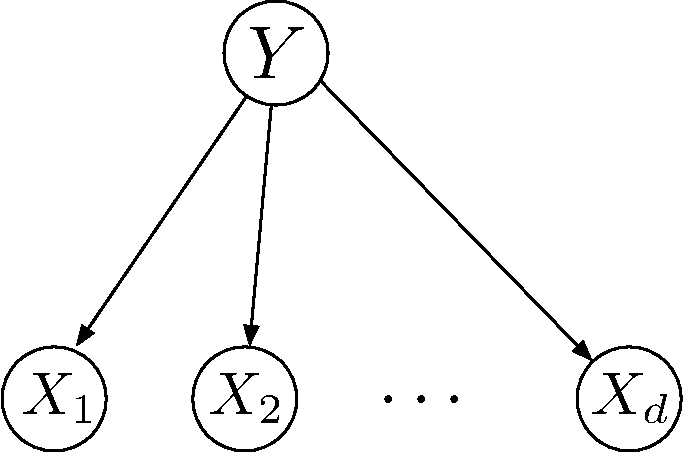
\includegraphics[width=0.3\linewidth]{figures/naivebayesgm}
\end{center}

As a motivating example, let's look back at the Titanic dataset from the last module.  A potential BN for the Titanic dataset is shown below.

\begin{center}
\includegraphics[width=0.8\linewidth]{figures/titanicbn}
\end{center}

The probabilities in this BN were computed by looking at the training set and counting the appropriate passengers that fell into each category.  For instance, to compute $p(\mathcal{Y}|\mathcal{S})$ since $p(\mathcal{Y}|\mathcal{S}) = \frac{p(\mathcal{Y}, \mathcal{S})}{p(\mathcal{S})}$, we can approximate this probability by counting the number of passengers under 5 who survived and dividing by the total number who survived (note that there are some subtle and important modifications to this method of fitting these probabilities that we'll discuss in the next assignment).  This process was repeated for each conditional probability.  Since we assume that all of the features are conditionally independent given the output ($\mathcal{S}$ in this case), this process is done independently for each feature.

\subsection{Inference}
While the Na\"ive Bayes Algorithm might sound fancy, once we have the BN, all we need to do to run the algorithm is to use Bayes' rule.  We'll let you work through this on your own via an exercise.

\begin{exercise}[(45 minutes)]

\bes
\item Using the BN shown above, what is the probability that a young, male in first class would survive the Titanic disaster?  Hint: write this as a conditional probability and then use Bayes' rule.  Hint 2: leverage the fact that $\mathcal{C}, \mathcal{Y}, \mathcal{M}$ are all conditionally independent of each other given $\mathcal{S}$.

You have just derived the Na\"ive Bayes inference rule!

\begin{boxedsolution}
\begin{align}
p(\mathcal{S}|\mathcal{Y}, \mathcal{C}=1, \mathcal{M}) &= \frac{p(\mathcal{Y}, \mathcal{C}=1, \mathcal{M}|\mathcal{S})p(\mathcal{S})}{p(\mathcal{Y}, \mathcal{C}=1, \mathcal{M})} \nonumber \\
&= \frac{p(\mathcal{Y}, \mathcal{C}=1, \mathcal{M}|\mathcal{S})p(\mathcal{S})}{p(\mathcal{Y}, \mathcal{C}=1, \mathcal{M}| \mathcal{S})p(\mathcal{S}) + p(\mathcal{Y}, \mathcal{C}=1, \mathcal{M}|\neg \mathcal{S})p(\neg \mathcal{S})} \nonumber \\
&=  \frac{p(\mathcal{Y}|\mathcal{S}) p( \mathcal{C}=1 | \mathcal{S}) p(\mathcal{M}|\mathcal{S})p(\mathcal{S})}{p(\mathcal{Y}|\mathcal{S}) p( \mathcal{C}=1 | \mathcal{S}) p(\mathcal{M}|\mathcal{S})p(\mathcal{S}) + p(\mathcal{Y}|\neg \mathcal{S}) p( \mathcal{C}=1 | \neg \mathcal{S}) p(\mathcal{M}|\neg \mathcal{S})p(\neg \mathcal{S})} \nonumber \\
&= \frac{\left ( \frac{27}{342} \times \frac{136}{342} \times \frac{109}{342}\times \frac{342}{891}\right)}{\left ( \frac{27}{342} \times \frac{136}{342} \times \frac{109}{342}\times \frac{342}{891} \right ) + \left ( \frac{13}{549} \times \frac{80}{549} \times \frac{468}{549}\times \frac{549}{891} \right )} \nonumber \\
&= 0.6794 \nonumber
\end{align}

\end{boxedsolution}

\item Na\"ive Bayes is often more conveniently expressed using odds ratios.  Instead of computing $p(\mathcal{S}|\mathcal{Y}, \mathcal{C}=1, \mathcal{M})$ let's compute the following.
\begin{align}
\frac{p(\mathcal{S}|\mathcal{Y}, \mathcal{C}=1, \mathcal{M})}{p(\neg \mathcal{S}|\mathcal{Y}, \mathcal{C}=1, \mathcal{M})} &= \frac{\frac{p(\mathcal{Y}, \mathcal{C}=1, \mathcal{M} | \mathcal{S})p(\mathcal{S})}{p(\mathcal{Y},\mathcal{C}=1, \mathcal{M})}}{\frac{p(\mathcal{Y}, \mathcal{C}=1, \mathcal{M} | \neg \mathcal{S})p(\neg \mathcal{S})}{p(\mathcal{Y},\mathcal{C}=1, \mathcal{M})}} \nonumber \\
&=  \frac{p(\mathcal{Y}, \mathcal{C}=1, \mathcal{M} | \mathcal{S})p(\mathcal{S})}{p(\mathcal{Y}, \mathcal{C}=1, \mathcal{M} | \neg \mathcal{S})p(\neg \mathcal{S})} \nonumber \\
&= \frac{p(\mathcal{Y} | \mathcal{S}) p(\mathcal{C}=1 | \mathcal{S}) p(\mathcal{M} | \mathcal{S})p(\mathcal{S})}{p(\mathcal{Y}| \neg \mathcal{S}) p(\mathcal{C}=1 | \neg \mathcal{S}) p(\mathcal{M} | \neg \mathcal{S})p(\neg \mathcal{S})} \nonumber
\end{align}

What must be true about this odds ratio in order to predict that the passenger survived?
\begin{boxedsolution}
The odds ratio must be greater than 1, which implies that
\begin{align}
p(\mathcal{S}|\mathcal{Y}, \mathcal{C}=1, \mathcal{M}) &> p(\neg \mathcal{S}|\mathcal{Y}, \mathcal{C}=1, \mathcal{M}) \enspace . \nonumber
\end{align}
\end{boxedsolution}

\ees
\end{exercise}



\section{Compas Model of Recidivism}


\end{document}
